\section{Umsetzung}
\label{sec-5}

Im folgenden soll erläutert werden, wie der zuvor erarbeitete Lösungsansatz umgesetzt wurde. Dazu gibt das Kapitel zunächst einen Überblick über das System und die Architektur der Anwendung. Nach einer kurzen Erläuterung zu ''Screen-Captures'' von der HoloLens folgt eine nähere Betrachtung dessen, wie die Hologramme umgesetzt wurden. Schließlich werden Details zur Interaktion und Performance genannt.

\subsection{Aufbau des Systems}
\label{sec-5-1}
Das System ist als Client-Server-Architektur realisiert, einen Überblick gibt das Schema in Abb. \ref{img:communication-schema}. Ein Server erfasst und verarbeitet die in der Schaltung gemessenen Werte für die Stromstärke. Diese stammen von einem Arduino, der in den Stromkreislauf eingekoppelt ist. Die Applikation auf der HoloLens tritt als Client auf und erfragt die aktuellen Werte vom Server. 
\begin{figure}[H]
	\centering
	\includegraphics[width=0.45\textwidth]{images/todo.jpg}
	\caption{Schema Kommunikation Schaltung Arduino Server HoloLens}
	\label{img:communication-schema}
\end{figure}

\subsubsection{Client-Server Datenübertragung}
\label{sec-5-1-1}
Die Übertragung der Messwerte vom Arduino zur Anwendung ist so konzipiert, dass Änderungen in Echtzeit übermittelt werden, ohne das unnötiger Netzwerktraffic entsteht. Der Client betreibt ein Polling gegen den Server, der jedoch Antworten solange zurückhält, bis ein neuer, vom vorigen abweichender Wert gemessen wurde. Dieses Verhalten veranschaulicht das Sequenzdiagramm in Abbildung \ref{img:Sequenzdiagramm}. Das Vorgehen führt dazu, dass Änderungen durch den Nutzer am Regler der Spannungsquelle ohne wahrnehmbare Verzögerung auf der HoloLens ankommen.

\vspace{8px}
\begin{center}
	\fbox{
		\parbox{0.9\linewidth}{
			\vspace{4px}
			\textbf{Überblick}
			\begin{itemize}[rightmargin=12px, topsep=-12px]
				\setlength{\itemsep}{-1pt}
				\singlespacing
				\item HoloLens erfragt Daten vom Server über HTTP GET-Requests
				\item Anfragen erfolgen asynchron
				\item Server nimmt den Request entgegen und hält eine Antwort solange zurück, bis ein neuer Wert vom Arduino vorliegt
				\item Dadurch kommen neue Daten sehr schnell bei der HoloLens an, der Nutzer sieht die Änderungen auf der Brille sofort, wenn er Änderungen an der Spannungsquelle vornimmt
				\item So wird zeitliche Einbettung und Kontinuität erreicht
				\item Dabei wird jedoch kein unnötiger Traffic erzeugt
			\end{itemize}
			\vspace{18px}
	}}\\
\end{center}
%\vspace{6px}

\begin{figure}[H]
	\centering
	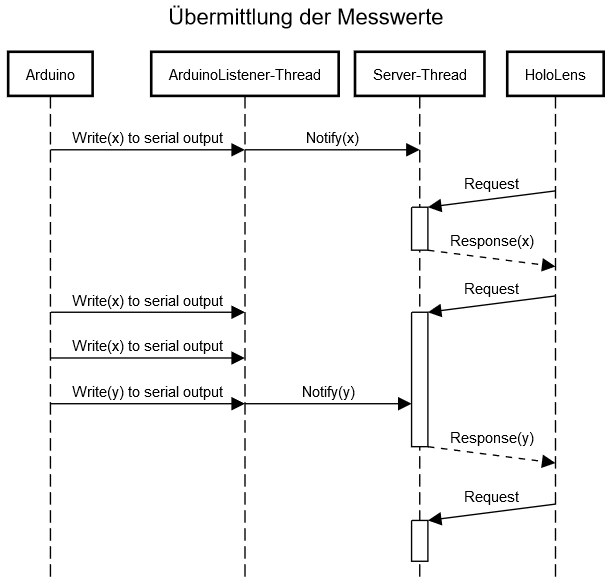
\includegraphics[width=0.8\textwidth]{images/schema/Sequenzdiagramm.png}
	\caption{Sequenzdiagramm Kommunikation}
	\label{img:Sequenzdiagramm}
\end{figure}

\textit{Server}\\
Der Server besteht aus zwei miteinander kommunizierenden Threads. Ein Thread übernimmt das Lesen und Verarbeiten der Rohdaten, die über die serielle Schnittstelle eintreffen. Bei signifikanten Änderungen wird der zweite Thread mittels einer gemeinsamen, synchronisierten Variablen über die neuen Werte informiert. Dieser beantwortet daraufhin einen ggf. ausstehenden Request vom Client. Ab wann eine Änderung als signifikant gewertet wird, lässt sich über einen Threshold einstellen. Der Server wurde mit Python und der Bibliothek pyserial umgesetzt.\\

\textit{Client}\\
Der Client stellt durch die Nutzung von asynchronen Anfragen sicher, dass die Anfragen nicht blockieren. Unity bietet nur einen Thread, synchrone Anfragen würden daher zu einer Blockierung des Renderprozesses führen und so die Framerate beeinträchtigen. Da die Framerate bei 60 Hz gedeckelt ist und eine Antwort frühestens im nächsten Frame bearbeitet werden kann, beträgt die minimale Antwortzeit ca. 17 ms. Das ist ausreichend, um keine wahrnehmbare Verzögerung aufkommen zu lassen, da die Paketlaufzeit in einem lokalen Netzwerk typischerweise im einstelligen Millisekundenbereich liegt. Eine zusätzliche Wartezeit zwischen Requests kann außerdem eingestellt werden.\\

\subsubsection{Architektur der HoloLens-Anwendung}
\label{sec-5-1-2}
Der Hauptteil des Systems besteht in der auf der HoloLens laufenden Applikation. Die Anwendung basiert auf der Unity Engine und wird als UWP App bereitgestellt. Das Schema in Abb. \ref{img:components-schema} gibt einen Überblick über die verschiedenen Komponenten der Anwendung. Deren Aufgaben sind in der darunter zu findenden Tabelle kurz zusammengefasst.

\begin{figure}[H]
	\centering
	\includegraphics[width=0.45\textwidth]{images/todo.jpg}
	\caption{Schema Komponenten}
	\label{img:components-schema}
\end{figure}


\vspace{8px}
\begin{center}
	\fbox{
		\parbox{0.9\linewidth}{
			\vspace{4px}
			\textbf{Überblick}	
\bgroup
\setlength\extrarowheight{-2pt}
\def\arraystretch{2}
\begin{table}[H]
	\centering
	\begin{tabular}{m{2.5cm}|m{8cm}}
		Komponente & Funktion\\
		\hline
		\hline
		Menu & Hauptmenü, steuert den Ablauf der Anwendung\\
		\hline
		Settings & Lädt und Speichert Einstellungen, bietet Zugang zu den Werten für andere Komponenten und steuert die Einstellungs-Oberfläche\\
		\hline
		Physics & Übernimmt alle physikalischen Berechnungen. Alle relevanten physikalischen Parameter lassen sich konfigurieren.\\
		\hline
		Tracking & Führt durch den Prozess der Positionsbestimmung und setzt den World Anchor\\
		\hline
		Model Anchor & Dient als Anker- und Container-Objekt für die einzelnen Darstellungskomponenten. Dazu gehören: Verdeckungsmodell, Kompass, die Magnetfeldmodelle, die Stromrichtungsindikatoren und das Datenpanel.\\
		\hline
		Webservice & Übernimmt die Kommunikation mit dem Server und gibt erhaltene Daten weiter\\
		\hline
		Interaction & Verarbeitet Input und Ablaufsteuerung, soweit dies nicht an einem konkreten Objekt abgewickelt wird wie z.B. Spracheingabe.\\
	\end{tabular}\caption{\label{tab:components-details} Aufgaben der einzelnen Komponenten}
\end{table}
\egroup
%\vspace{18px}
}}\\
\end{center}
\vspace{6px}

Eine Komponente besteht aus einer Hierarchie von Unity's GameObjects, die mit entsprechenden Skripten versehen sind. Die Komponenten kommunizieren auf unterschiedliche Weise miteinander. Die Behandlung von Events z.B. aufgrund von Nutzereingaben oder neuen Messwerten erfolgt über Callbacks. Manche Komponenten sind auch Singletons, auf die direkt zugegriffen werden kann wie z.B. die Einstellungen.

\subsection{Implementierung}
\label{sec-5-2}

\subsubsection{Implementierung der Darstellungen}
\label{sec-5-2-2}
Nachdem die grundlegende Architektur der vorgestellt wurde folgt nun eine genauere Betrachtung der Umsetzung der Darstellungen. Die Ausführungen werden dabei durch Abbildungen in Form von Screenshots unterstützt. Einen ersten Eindruck vermitteln die Fotos in Abb. \ref{img:HL_SS_Intro}. Damit die von der HoloLens stammenden Bilder richtig interpretiert werden können, sind jedoch einige Vorbemerkungen nötig.

\begin{figure}[h!]
	\centering
	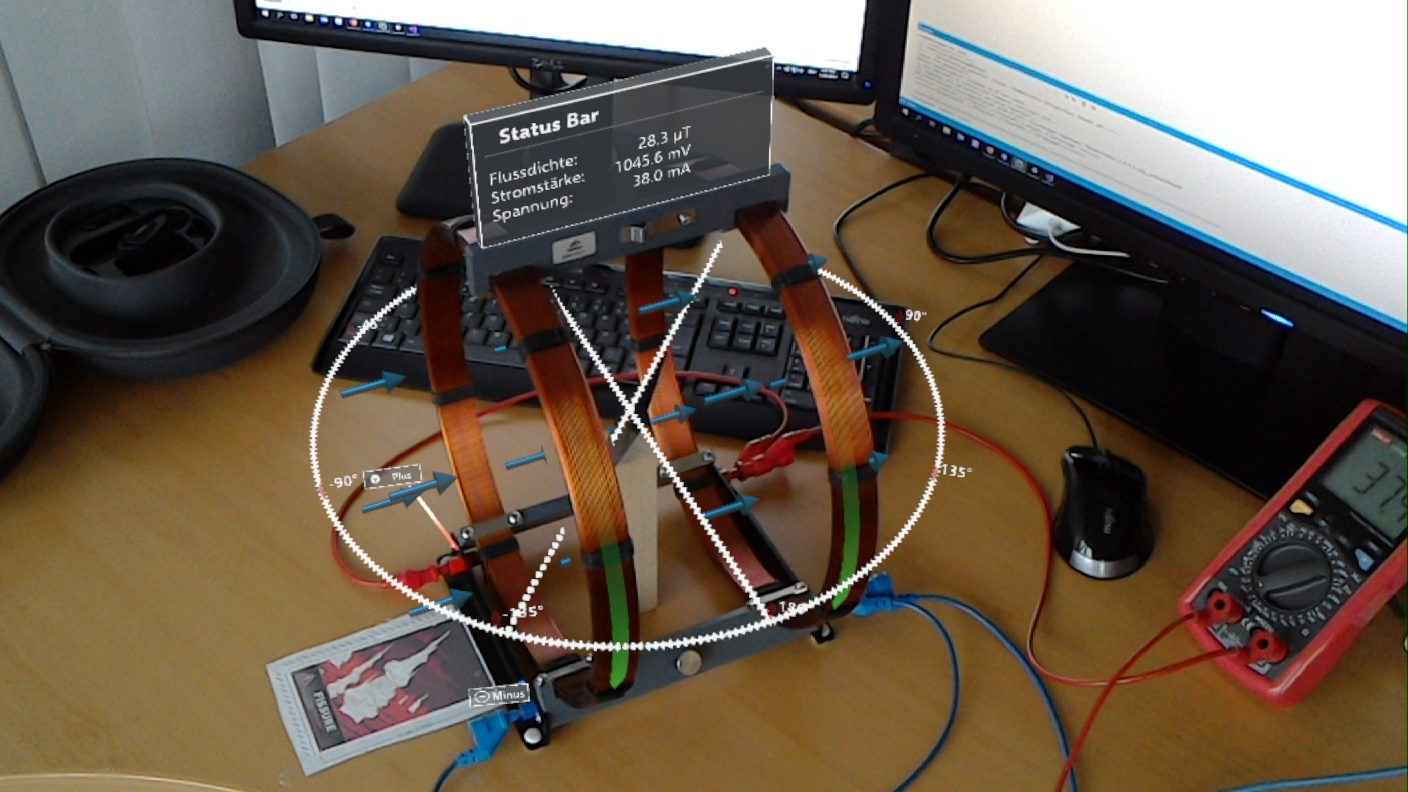
\includegraphics[width=\textwidth]{images/HL_SS1.jpg}

	\vspace{0.25cm}

	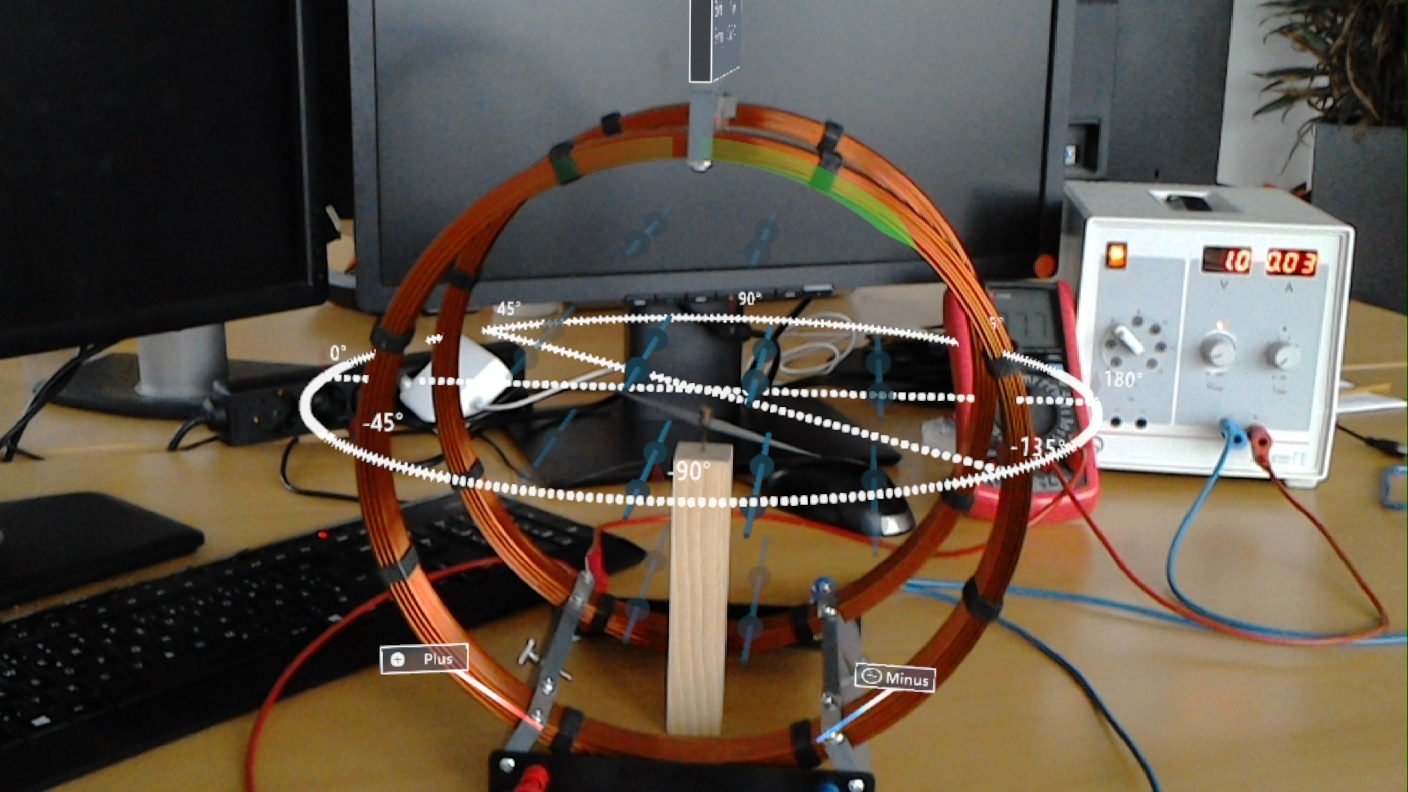
\includegraphics[width=\textwidth]{images/HL_SS2.jpg}
	\caption{Erster Eindruck HoloLens}
	\label{img:HL_SS_Intro}
\end{figure}

Die Qualität von Aufnahmen mit der HoloLens ist deutlich eingeschränkt und weicht von der tatsächlichen Nutzererfahrung ab. Die wesentlichen Einschränkungen sind dabei: 
\begin{itemize}
	\setlength{\itemsep}{-1pt}
	\singlespacing
	\item Andere Auflösung mit geringerer Pixeldichte
	\item Stark vergrößertes Sichtfeld
	\item Verfälschte Farben und Transparenzen
	\item Verfälschte Positionierung
	\item Aufnahmen nicht möglich, wenn Kamera durch Anwendung genutzt wird
\end{itemize}

\textit{Echtzeitdarstellungen des Magnetfeldes}\\
Die Darstellung des Magnetfeldes in Echtzeit erfolgt über 3D-Objekte. Die Geometrie wurde mit Blender erstellt und in Unity importiert.

\textit{Vorberechnete Darstellung des Magnetfeldes}\\
\begin{itemize}[rightmargin=12px, topsep=-12px]
	\setlength{\itemsep}{-1pt}
	\singlespacing
	\item Feldlinien vorberechnet mit COMSOL Multiphysics, exportiert als CSV, Import in Unity erfolgt zur Laufzeit
	\item Maximale Qualitätseinstellungen in Simulationssoftware um Artefakte durch numerische Ungenauigkeiten zu vermeiden
	\item Filtering beim Import auf der HoloLens reduziert Datenpunkte für Performance
\end{itemize}

Die numerische Lösung der Feldgleichungen erfolgte mittels der Simulationssoftware COMSOL Multiphysics. Diese Arbeit konnte hier auf eine bestehende Implementierung einer Helmholtzspule aufbauen. Hier wurden lediglich die folgenden Parameter für die Berechnung der Feldlinien gesetzt:
\begin{itemize}
	\setlength{\itemsep}{-1pt}
	\singlespacing
	\item Volumen für Begrenzung der Simulation: 2 Meter, maximale Granularität
	\item 12 Feldlinien, Startpunkte der Simulation auf der X-Achse
	\item Qualitätseinstellungen der Darstellung auf Maximum gesetzt
\end{itemize}

\textit{Export, Import, Datenformat}\\
Das Ergebnis der Simulation ist eine Liste von Datenpunkten der Form \textbf{[}\textit{FeldlinienNr:} Int, \textit{Position:} Vector3, \textit{Betrag der Flussdichte:} float\textbf{]}. Dafür wurde ein CSV-Reader geschrieben, der die Daten zur Laufzeit der Applikation einliest, interpretiert und zum Rendering an GameObjects weitergibt. Folglich ließen sich weitere Simulationen vorberechnen und anzeigen. Einlesen der Daten erfolgt beim Startvorgang.\\

\textit{Filtering}\\
Entfernen doppelter Linien, Minimum-Abstands-Kriterium, Ursprünglich ca. 12k Datenpunkte, Reduktion um ca. 90\% 

\textbf{Stromfluss}
Die Indikatoren werden dynamisch über ein Skript erzeugt und gesteuert. Hier können Parameter wie Richtung, Position, Radius und Bogenlänge festgelegt werden. Die Breite der Linien wurde auf 1cm gesetzt. Die Größe ist für die gewünschte Entfernung ausreichend und übersteigt die Dicke der Spulen nicht. Indem die Darstellung sich der Betrachtungsposition kontinuierlich anpasst wird der Nutzer zusätzlich in die Anwendung einbezogen.\\

\textit{Strom-Labels}\\
Hier konnte auf ein vorgefertigtes Tooltip-Objekt des MRTK zurückgegriffen werden. Diese wurden um die entsprechenden Farben und Icons ergänzt. Die Icons basieren auf freien Icon-Packeten \footnote{https://icons8.com}, wurden jedoch angepasst. Da schwarze Strukturen vor transparentem Grund auf der HoloLens so nicht zu sehen sind, wurde der Hintergrund bzw. die Icon-Struktur zu weiß geändert.\\

\textbf{Kompass}\\
2D-Linien mit Unity's LineRenderer. Gestrichelte Linie durch Textur mit weißem Kreis und transparentem Hintergrund, Skalierung auf die Länge der Linie mit Tiling. Eigenes Skript dafür.

\textbf{Datenpanel und weitere Informationen}\\
Die weiteren, optional einblendbaren Informationen wie Spulenabstand oder Windungszahl wurden aus zeitlichen Gründen nicht umgesetzt, da hier eine weitere Interaktionsmöglichkeit einzurichten wäre, um die Elemente ein- und auszublenden.


\textit{Occlusion Berechnung}\\
Für die Verdeckungsberechnung wurde die Spule anhand gemessener Größen in Blender modelliert. Das Spatial Mapping der HoloLens ist hier zu ungenau, um eine glaubwürdige Verdeckung zu ermöglichen. In der Standard-Einstellung wird die Spule gar nicht erkannt, was wohl auch dem Material (Kupfer) geschuldet sein dürfte. Eine Darstellung des Spatial Mappings des Versuchsaufbaus ist in Abb. \ref{img:mesh-vs-model} zu sehen.
\begin{figure}[H]
	\centering
	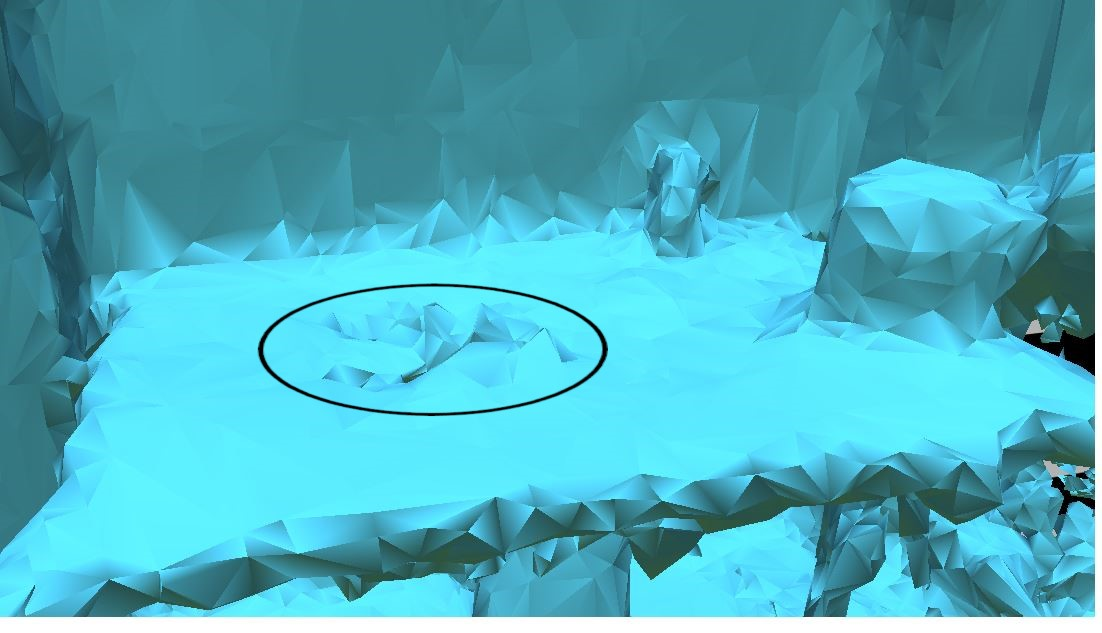
\includegraphics[width=0.45\textwidth]{images/HL/mesh.jpg}
	\caption{Spatial Mapping der Gerätschaften. Während die Spannungsquelle gut zu sehen ist, ist die Spule lediglich als Unebenheiten im Tisch zu erkennen.}
	\label{img:mesh-vs-model}
\end{figure}
Die Geometrie wird ausschließlich in den Tiefenpuffer gerendert\footnote{Der entsprechende Shader ist nur wenige Zeilen lang und findet sich in verschiedenen Varianten im Internet. Dieser orientiert sich an http://wiki.unity3d.com/index.php/DepthMask}. Das vermeidet überflüssige Draw Calls und folgt der Empfehlung der Dokumentation. Damit virtuelle Objekte aber auch dann noch verdeckt bleiben, wenn reale Objekte nah kommen, muss das Near Clipping Plane sehr nah am Kameraursprung liegen. Andernfalls würden weiter entfernte, virtuelle Objekte plötzlich doch vor realen Objekten angezeigt werden, sobald letztere zu nah sind und das Clipping die für die Verdeckung eingesetzten Objekte vom Rendering ausschließt. Das stellt bei dieser Lösung aber kein Problem dar, weil zu nahe, virtuelle Objekte ohnehin über ein eigenes Verhalten ausgeblendet werden, das nicht auf die Clippingebene aufbaut.\\


\textit{Near Plane Fading}\\
Anstelle auf Basis der Clippingebene werden zu nahe Objekte über Skripte bzw. Shader kontinuierlich ausgeblendet. Dieses Verhalten ist für den Nutzer angenehmer als ein plötzliches Aufpoppen bzw. Verschwinden von Objekten in unmittelbarer Nähe.\\

Der für die meisten Objekte genutzt MRTK Standard Shader bietet bereits einen konfigurierbaren Bereich, über den Objekte ausgeblendet werden. Für andere Elemente wird die Transparenz über ein Skript geregelt. Hier werden für Anfang und Ende des Bereiches, über den zur Transparenz übergegangen wird, die empfohlenen Werte von 85cm und 50cm genutzt. Lediglich die Linien des Kompasses werden 10 cm ''später'' ausgeblendet, damit die Ausrichtung der Nadel entlang der Linien auch aus geringerem Abstand und damit etwas besser erfasst werden kann. Insgesamt ergibt sich die Transparenz (Alpha-Wert) eines Objektes dann aus dem Minimum der Werte durch die verschiedenen Effekte.\\

Diese Lösung geht jedoch zu Lasten der Performance, denn für die Transparenz werden alle betroffenen Objekte von hinten nach vorne (aus Sicht der Kamera) gerendert. Auch Pixel, die durch weiter vorne gelegene Objekte eingenommen werden, müssen mehrfach gezeichnet werden, da die dichteren Objekte ggf. transparent sind und durch die Farbe anderer Objekte beeinflusst werden. Dieser sogenannte Overdraw nimmt zusätzliche Rechenzeit in Anspruch. Eine Alternative bestünde darin, Objekte schwarz anstatt transparent werden zu lassen. Auf der HoloLens macht dies optisch zunächst keinen Unterschied, da Schwarz auf der Brille nicht dargestellt wird. Allerdings bliebe so die Verdeckung durch bereits verschwundenen Objekte bestehen, was zu Irritationen führen würde.\\

\textit{Kantenglättung}\\
Bei Darstellungen auf der HoloLens fällt der Kantenglättung eine besondere Bedeutung zu. Im Gegensatz zu anderen Anwendungen, bei denen der Nutzer die Kamera über herkömmliche Eingabegeräte steuert, ist bei der Brille die Kamera an die Kopfbewegungen des Trägers gebunden. Die Displays folgen daher den ständigen, feinen Vibrationen des Kopfes und die Kamera steht somit nie still. Deshalb können Treppeneffekte an Kanten besonders auffällig und störend wirken, da das resultierende Kantenflimmern stetig präsent ist.\\

Unity unterstützt standardmäßig einige Anti-Aliasing Verfahren. Dazu gehört Multisample Anti-Aliasing (MSAA), das ohne weitere Maßnahmen für die Kamera aktiviert werden kann. Im Gegensatz dazu benötigen die anderen Methoden\footnote{Standardmäßig angeboten werden außerdem Fast Approximate AA und Temporal AA} Deferred Shading und würden eine Umstellung des Rendering Path bedeuten. Im Rahmen dieser Arbeit wurde deshalb nur MSAA in Betracht gezogen.\\

Vor allem für die gewählte Visualisierung der Simulationsdaten über Linien ist eine Form des Anti-Aliasing relevant, da hier besonders viele Kanten entstehen. Deshalb wurde sich für Einsatz von zweifachem MSAA entschieden, obwohl damit erheblicher Rechenaufwand verbunden ist.\\

\textit{Künstliche Beleuchtung}\\
Beleuchtung bildet grob erwartete Lichtverhältnisse nach, keine Schatten
\begin{itemize}
	\item Virtuelle Beleuchtung von Oben bildet echte Lichtverhältnisse grob nach
	\item Unterstützt die Einbettung der 3D Objekte im Raum
\end{itemize}


\subsection{Implementierung der Interaktion}
\begin{itemize}[rightmargin=12px, topsep=-12px]
	\setlength{\itemsep}{-1pt}
	\singlespacing
	\item Tracking mit Vuforia, nur zum Erkennen des Markers aktiv
	\item Einstellungen werden als JSON-Datei im AppData Verzeichnis gespeichert
	\item Menü übernimmt Steuerung der einzelnen Vorgänge, jederzeit aufrufbar
	\item Startvorgang mit Intro-Sequenz lädt Daten und Einstellungen und initialisiert Komponenten
\end{itemize}
Die Interaktion erfolgt, wie in Kap. \ref{sec-4-4} beschrieben, durch Klicks. Sprachbefehle wurden aus Zeitgründen nur für Debugging-Funktionen implementiert. 
Während des Hauptteils der Anwendung belaufen sich die möglichen Aktionen auf:

\begin{itemize}
	\setlength{\itemsep}{-1pt}
	\singlespacing
	\item Klick: Wechsel zwischen den beiden Echtzeitdarstellungen
	\item Doppelklick: Wechsel zwischen Simulations- und Echtzeitdarstellungen
	\item Hold-Klick: Aufrufen des Hauptmenüs
\end{itemize}

Für die letzteren beiden wurden entsprechende Skripte geschrieben, die diese Gesten erkennen. Zwar erkennt das MRTK bereits eine Hold-Geste, allerdings kann hier der Nutzer beliebig lange gedrückt halten und erst beim Loslassen feuert das entsprechende Event. Zum Aufrufen des Menüs ist jedoch ein Verhalten wünschenswert, bei dem nach kurzem Gedrückt-Halten das Menü erscheint. Daher wurde hier eine eigene Lösung entwickelt.\\

Jeder Klick wird durch einen Klick-Sound begleitet, der als Feedback dient. Ist der Cursor aktiv, bietet dieser auch ein visuelles Feedback. Als Klick-Sound wurde ein Standard-Sound des MRTK verwendet, der auch von den Buttons genutzt wird.

\textit{Progress Indikator}\\
Um den Anwender über länger laufende Prozesse zu informieren, kommt eine Fortschrittsanzeige zum Einsatz. Hier kann auf den aus Mircosoft Windows bekannten Indikator zurückgegriffen werden, den das MRTK als vorgefertigtes Objekt anbietet. Das Mixed Reality Capture in Abb. \ref{img:pi-and-tracking} zeigt diesen beim Start der Anwendung.\\

\begin{figure}[H]
	\centering
	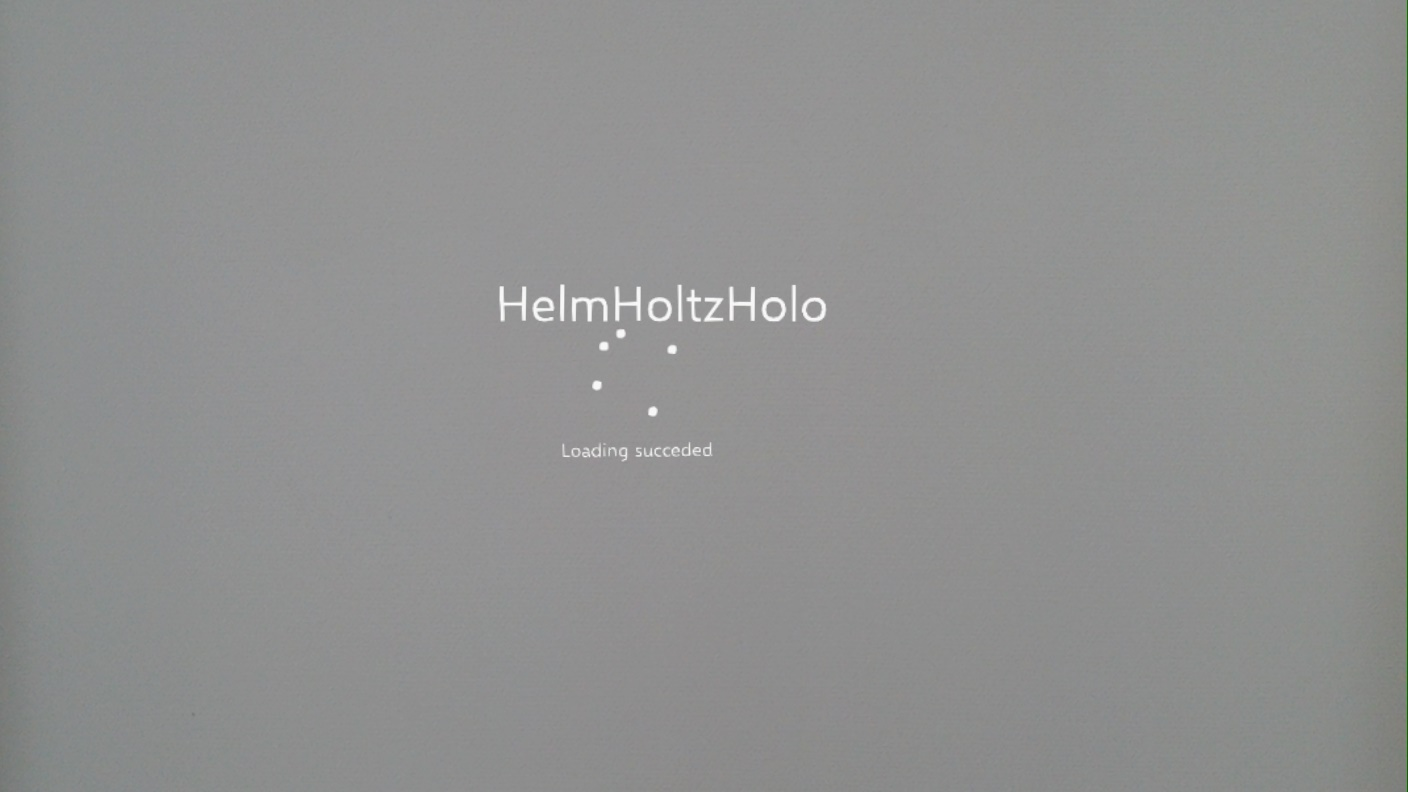
\includegraphics[width=0.45\textwidth]{images/loading.jpg}
	\hspace{0.05cm}	
	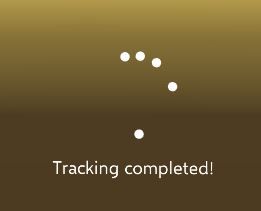
\includegraphics[width=0.45\textwidth]{images/tracking.jpg}
	\caption{Progress Indikator Laden und Tracking}
	\label{img:pi-and-tracking}
\end{figure}

Für die Kommunikation mit dem Nutzer ist bei dieser Anwendung vor allem wichtig, was das System tut. Längere Ladezeiten o.Ä. treten hier nicht auf, daher wird lediglich das Text-Element des Indikators verwendet, von der prozentualen Anzeige wird nicht Gebrauch gemacht. Komponenten, die den Indikator nutzen, stellen jedoch stets sicher, dass eine Nachricht lange genug sichtbar ist, um gelesen werden zu können. Länger laufende Operationen sind stets asynchron umgesetzt, die pro Frame nur einen Teil der Arbeit erledigen und so den Renderprozess nicht blockieren.\\

\textit{Tracking}\\
Für das Erkennen der Markerposition kommt das Tracking Framework Vuforia zum Einsatz. Ein optischer Marker wird vor der Spule auf dem Untergrund platziert. Dieser wird dann über die Frontkamera der HoloLens durch das Framework erkannt und die Position und Ausrichtung bestimmt. Die Modelle werden entsprechend positioniert und ein World Anchor gesetzt. Damit ist die Positionierung abgeschlossen und der Marker kann entfernt werden. Da Vuforia nur während dieser Sequenz aktiviert ist, werden für den Rest der Anwendung Hardwareressourcen frei.\\

Dieser Vorgang lässt sich über das Menü jederzeit neu anstoßen und die einzelnen Schritte werden über den Progress Indikator dem Nutzer kommuniziert. Die Steuerung des Prozesses erfolgt durch den \textit{Tracking Manager}. Dieser startet und stoppt das Framework, reagiert auf Änderungen im Tracking und informiert den Anwender über den Fortschritt. Der Screenshot\footnote{Wie in Kap. \ref{sec-5-2-1} festgehalten sind während des Trackings keine Aufnahmen mit der HoloLens möglich, da die Kamera von Vuforia in Anspruch genommen wird.\nopagebreak} in Abb. \ref{img:pi-and-tracking} zeigt eine solche Nachricht.\\

\textit{Einstellungen}\\
Die Einstellungen sind über ein dem Daten-Panel ähnliches Objekt realisiert, das in Abb. \ref{img:menu-and-settings} zu sehen ist. Ein Klick auf eines der Input-Felder ruft die virtuelle Tastatur hervor, beide werden durch das MRTK bereitgestellt und wurden hier für numerische Eingaben konfiguriert. Die Werte werden als JSON formatiert und in das AppData-Verzeichnis der Anwendung gespeichert. Damit stehen sie auch nach einem Neustart oder Update der App noch zur Verfügung. Die Applikation sucht beim Start automatisch nach gespeicherten Einstellungen und lädt entweder diese oder die Default-Werte. Andere Komponenten werden durch ein Event über sich ändernde Einstellungen benachrichtigt und passen sich entsprechend an.\\

\begin{figure}[H]
	\centering
	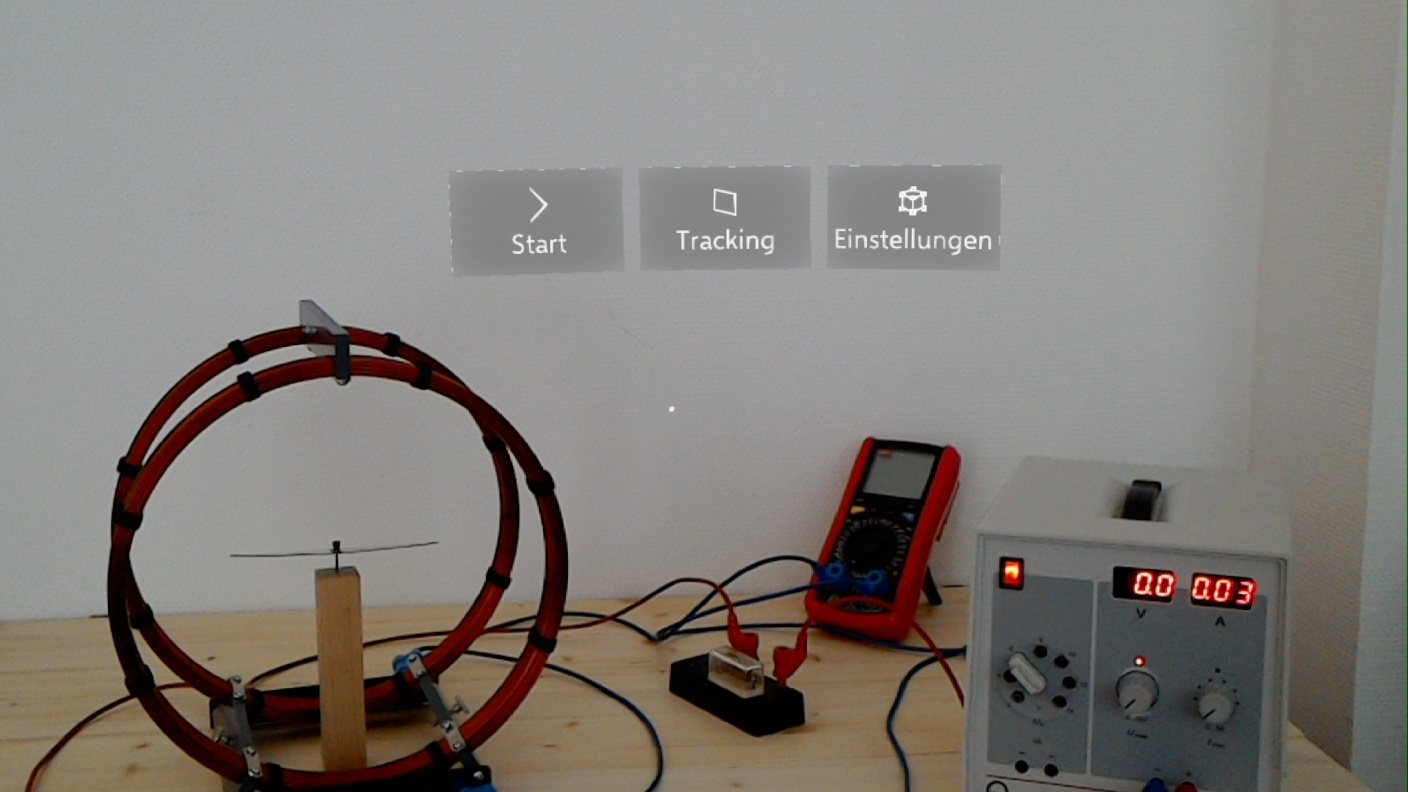
\includegraphics[width=0.45\textwidth]{images/menu.jpg}
	\hspace{0.05cm}	
	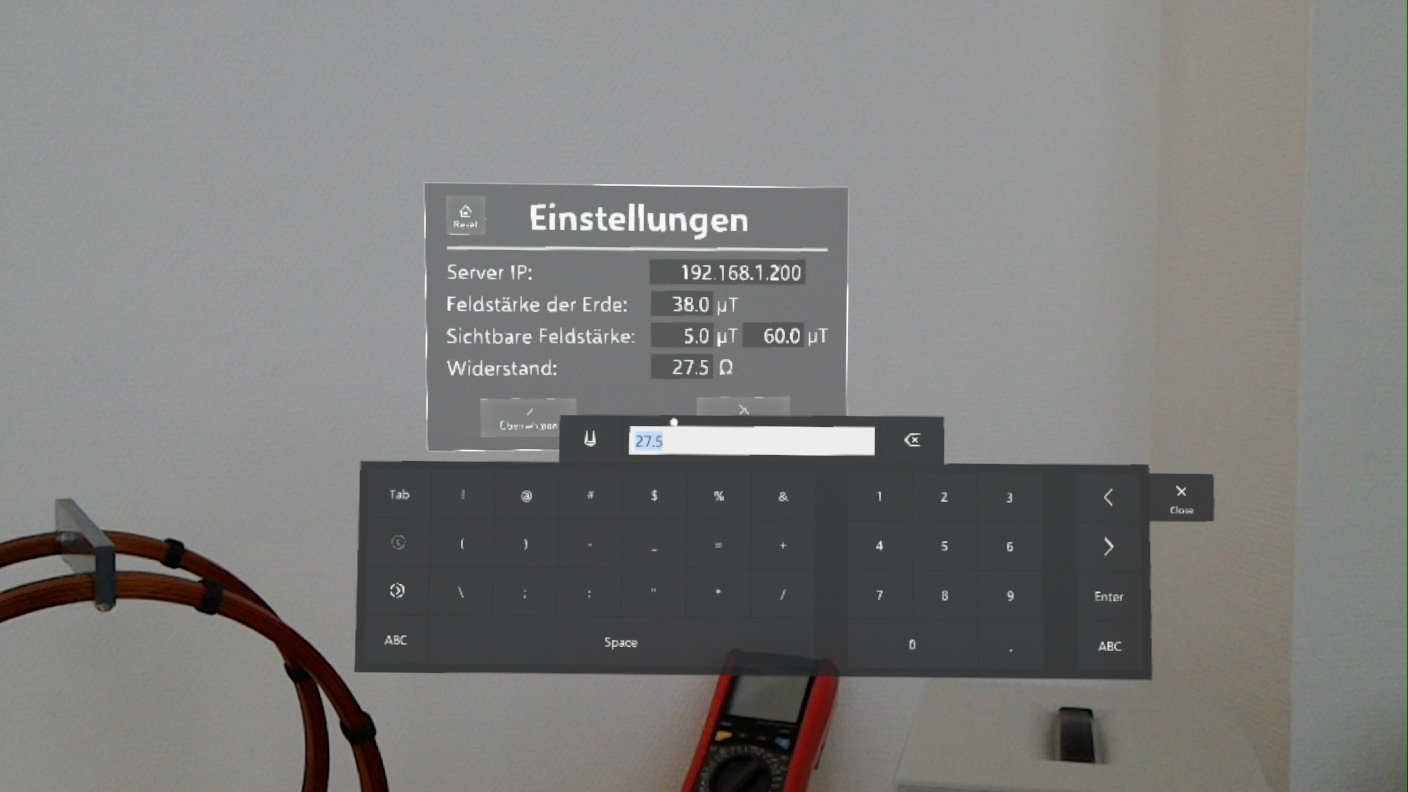
\includegraphics[width=0.45\textwidth]{images/settings.jpg}
	\caption{Einstellungen und Menü}
	\label{img:menu-and-settings}
\end{figure}

\textit{Menü}\\
Die Umsetzung des Menüs ist in Abb. \ref{img:menu-and-settings} abgebildet. Die Form der Buttons wurde so angepasst, dass die Labels und Icons problemlos darauf Platz finden. Bei den Icons wurde auf Standard-Elemente aus dem MRTK zurückgegriffen. Das Menü wird über den \textit{MenuController} gesteuert, von dem aus alle weiteren Vorgänge gestartet werden. Dieser aktiviert auch den Cursor, der zur Nutzung von Menu und EInstellungen dient.\\

\textit{Intro-Sequenz}\\
Es wurde eine Startsequenz entwickelt, die Aufgaben wie das Laden von Daten und Einstellungen und die Initialisierung der einzelnen Komponenten übernimmt. Hier wird ein Logo in Form eines größeren Schriftzuges und dazu der Progress Indikator angezeigt. Letzterer informiert über den Zustand des Ladevorgangs. Während des Vorgangs werden insbesondere die Einstellungen und  Simulationsdaten geladen.\\

Diese Umsetzung erlaubt die notwendigen Ladevorgänge und ist für den Nutzer nachvollziehbar. Außerdem gibt das letzterem einige Sekunden Zeit, um sich auf die Anwendung einzustellen, bevor das Menü erscheint und eine Aktion vom Anwender verlangt.

\subsection{Performance}
Zuletzt sollen einige Maßnahmen genannt werden, die zu einem geringeren Ressourcenverbrauch der Applikation beitragen. Zunächst ist festzuhalten, dass die durch das MRTK voreingestellten Qualitätseinstellungen genutzt wurden. Einzige Ausnahme stellt hier die Kantenglättung dar. Darüber hinaus wurden die folgenden Einstellungen angewandt:

\begin{itemize}
	\setlength{\itemsep}{-1pt}
	\singlespacing
	\item Single Pass Instanced Rendering
	\item Größe des Tiefenpuffers auf 16-Bit gesetzt (Minimum)
	\item Vuforia nur für den Vorgang der Positionsbestimmung aktiv
	\item Physics Enginge deaktiviert
	\item Occlusion Mesh wird ausschließlich in Z-Puffer gerendert
	\item Unsichtbare (vollst. transparente) Objekte werden meist deaktiviert
	\item Reduktion der Simulationsdaten auf ca. 10\% durch eine Minimum-Abstand-Regel und Bereinigung von doppelt gezeichneten Linien
\end{itemize}

Diese Maßnahmen basieren vorrangig auf den Empfehlungen zur Performance in der Dokumentation.